% interactcadsample.tex
% v1.03 - April 2017

\documentclass[]{interact}

\usepackage{epstopdf}% To incorporate .eps illustrations using PDFLaTeX, etc.
\usepackage{subfigure}% Support for small, `sub' figures and tables
%\usepackage[nolists,tablesfirst]{endfloat}% To `separate' figures and tables from text if required

\usepackage{natbib}% Citation support using natbib.sty
\bibpunct[, ]{(}{)}{;}{a}{}{,}% Citation support using natbib.sty
\renewcommand\bibfont{\fontsize{10}{12}\selectfont}% Bibliography support using natbib.sty

\theoremstyle{plain}% Theorem-like structures provided by amsthm.sty
\newtheorem{theorem}{Theorem}[section]
\newtheorem{lemma}[theorem]{Lemma}
\newtheorem{corollary}[theorem]{Corollary}
\newtheorem{proposition}[theorem]{Proposition}

\theoremstyle{definition}
\newtheorem{definition}[theorem]{Definition}
\newtheorem{example}[theorem]{Example}

\theoremstyle{remark}
\newtheorem{remark}{Remark}
\newtheorem{notation}{Notation}

% see https://stackoverflow.com/a/47122900


\usepackage{hyperref}
\usepackage[utf8]{inputenc}
\def\tightlist{}
\usepackage[usenames,dvipsnames]{color}
\newcommand{\er}[1]{\textcolor{Plum}{#1}}
\newcommand{\svp}[1]{\textcolor{Green}{#1}}
\newcommand{\rh}[1]{\textcolor{Orange}{#1}}

\begin{document}

\articletype{JSM 2021 Student Paper Competition (ASA sections on Statistical
Computing and Statistical Graphics)}

\title{Perception of exponentially increasing data displayed on a log scale}


\author{\name{Emily A. Robinson$^{a}$, Reka Howard$^{a}$, Susan VanderPlas$^{a}$}
\affil{$^{a}$Department of Statistics, University of Nebraska - Lincoln,}
}

\thanks{CONTACT Emily A. Robinson. Email: \href{mailto:emily.robinson@huskers.unl.edu}{\nolinkurl{emily.robinson@huskers.unl.edu}}, Reka Howard. Email: \href{mailto:rekahoward@unl.edu}{\nolinkurl{rekahoward@unl.edu}}, Susan VanderPlas. Email: \href{mailto:susan.vanderplas@unl.edu}{\nolinkurl{susan.vanderplas@unl.edu}}}

\maketitle

\begin{abstract}
Log scales are often used to display data over several orders of
magnitude within one graph. During the COVID pandemic, we've seen both
the benefits and the pitfalls of using log scales to display data. This
paper aims to\ldots{}
\end{abstract}

\begin{keywords}
Exponential; Log; Visual Inference; Perception
\end{keywords}

\hypertarget{introduction-and-background}{%
\section{Introduction and
Background}\label{introduction-and-background}}

\textcolor{Plum}{Graphics are a useful tool for displaying and communicating information. \citep{vanderplas2020testing}
Researchers include graphics to communicate their results in scientific publications and news sources rely on graphics to convey news stories to the public.}
\textcolor{Green}{May want to ask Heather about this one during the meeting (or by email)?}
\textcolor{Plum}{During the onset of the novel coronavirus pandemic, we saw an influx of dashboards being developed to display case counts, transmission rates, and outbreak regions \citep{lisa_charlotte_2020}.
People began subscribing to news sources involved in graphically tracking the coronavirus as a direct result of these pieces of work and the need for continually updated information \citep{rost_2020}; thus, gaining more exposure to the use of graphics.
}
\textcolor{Plum}{Many of these graphics helped guide decision makers to implement policies such as shut-downs or mandated mask wearing.
Also, these graphics helped officials communicate why policies were being enacted, with the hope of increasing population compliance.}
\textcolor{Green}{-- not sure what to cite, but the communication part can't be understated.}
\textcolor{Plum}{With the increasing importance graphics play in our everyday choices, we must actively choose which of many possible graphics to draw. 
Better sofware has mean easier and more flexible drawing allowing us to make design choices that best communicate the message of the data graphically, but as a result, we must consciously choose a set of principles to guide design choices in order to ensure that our charts are effective \citep{unwin_why_2020}.}

\textcolor{Plum}{
When faced with data which spans several orders of magnitude, we must decide whether to show the data on its original scale (compressing the smaller magnitudes into relatively little area) or to transform the scale and alter the contextual appearance of the data.
One common solution is to use a log scale transformation to display data over several orders of magnitude within one graph.
Logarithms make multiplicative relationships additive, showing elasticities and other proportional changes, and also linearize power laws \citep{menge_logarithmic_2018}. 
When presenting log-scaled data, it is possible to use either untransformed scale labels (for example, values of 1, 10 and 100 are equally spaced along the axis) or log-transformed scale labels (for example, 0, 1, and 2, showing the corresponding powers of 10).
}

\textcolor{Plum}{We have recently experienced the benefits and pitfalls of using log-scales as covid-19 dashboards displayed case count data on both the log and linear scale \citep{wade_fagen_ulmschneider_2020}. 
In spring 2020, during the early stages of the coronavirus pandemic, there was a large magnitude discrepancy at a given time between different geographic regions (at all orders of magnitude - states and provinces as well as countries and continents). 
During this time, we saw the usefulness of log-scales showing case count curves for areas with few cases and areas with many cases within one chart.
As the pandemic evolved, and the case counts were no longer spreading exponentially, graphs with linear scales seemed more effective at spotting early increases in case counts that signaled more localized outbreaks.
}

\textcolor{Plum}{
This is only one recent example of a situation in which both log and linear scales are useful for showing different aspects of the same data; there are long histories of using log scales to display results in ecology, psychophysics, engineering, and physics 
\citep{xkcd, menge_logarithmic_2018}.
}
\textcolor{Green}{XXX it may be interesting to find papers objecting to the use of log scales in some other disciplines beyond ecology.}

\textcolor{Plum}{
Research suggests our perception and mapping of numbers to a number line is logarithmic at first, but transitions to a linear scale later in development, with formal mathematics education.
This transition to linear scales occurs first in small numbers (e.g. 1-10) and then gradually expands to higher orders of magnitude; thus, the logarithmic intuition about numbers in children is often more noticeable on scales in the thousands to hundreds of thousands. \citep{varshney_why_2013, siegler_numerical_2017, dehaeneLogLinearDistinct2008}.
If we percieve logarithmically by default, it is a natural (and presumably low-effort) way to display information and should be easy to read and understand/use.}
\textcolor{Plum}{In fact, early studies explored the estimation and prediction of exponential growth, finding that growth is underestimated when presented both numerically and graphically but that numerical estimation is more accurate than graphical estimation for exponential curves.
One way to improve estimation of increasing exponential trends other than changing the scale is through the use of providing immediate feedback \citep{mackinnon_feedback_1991}.
While prior contextual knowledge or experience with exponential growth does not improve estimation, previous instruction on exponential growth reduces the underestimation by adjusting the initial starting value but not adjusting their perception of growth rate
\citep{wagenaar_misperception_1975, jones_polynomial_1977}.
Estimation was shown to improve when subjects were presented with decreasing exponential functions \citep{timmers_inverse_1977}.
\cite{jones_polynomial_1977}, \cite{wagenaar_extrapolation_1978}, and \cite{jones_generalized_1979} propose competing polynomial models for the perception and extrapolation of exponential series.
It seems that estimation is a two-stage process: first, we identify the type of curve and direction and then, we use that information for prediction \citep{best_perception_2007}.
}

\textcolor{Plum}{Our inability to accurately predict exponential growth might also be addressed by log-transforming the data, however, this transformation introduces new complexities: most readers are not mathematically sophisticated enough to intuitively understand logarithmic math and translate that back into real-world effects.
In \cite{menge_logarithmic_2018}, ecologists were surveyed to determine how often ecologists encounter log-scaled data and how well ecologists understand log-scaled data when they see it in the literature. 
Participants were presented two relationships displayed on linear-linear scales, log-log scales with untransformed values, or log–log scales with log-transformed values. 
\cite{menge_logarithmic_2018} propose three types of misconceptions participants encountered when presented data on log-log scales: 'hand-hold fallacy', 'Zeno's zero fallacy', and 'watch out for curves fallacies'. 
The 'hand-hold falacy' stems from the misconception that steeper slopes in log-log relationships are steeper slopes in linear-linear space. 
In fact, it is not only the slope that matters, but also the intercept and the location on the horizontal axis since a line in log-log space represents a power law in linear-linear space (i.e. linear extraploation). 
Emerging from 'Zeno's zero fallacy' is the misconception that positively sloped lines in log-log space can imply a non-zero value of y when x is zero. This is never true as postively sloped lines in log-log space actually imply that y = 0 when x = 0. 
This misconception again is a result of linear extrapolation assuming that a line in log-log space represents a line instead of the power law in linear-linear space. 
The last misconception, 'watch out for curves fallacies' encompases three faults: (1) lines in log-log space are lines in linear-linear space, (2) lines in log-log space curve upward in linear-linear space, and (3) curves in log-log space have the same curvature in linear-linear space. 
Linear extrapolation is again responsible for the first and third faults while the second fault is a result of error in thinking that log-log lines represent power laws (which are exponential relationships), and all exponential relationships curve upward; this is only true when the log-log slope is greater than 1.
\cite{menge_logarithmic_2018} found that in each of these scenarios, participants were consideraly confident in their incorrect responses indicating a incorrect knowledge rather than a lack of knowledge providing affirmation that our graphical design choices have a direct impact on the user's evaluation of the information.
}

\textcolor{Plum}{
In order to provide a set of principles to guide design choices, we must evaluate these design choices through the use of graphical tests. We can ask for participants to read information off of a chart and make effective decisions, we can ask participants to make predictions by e.g. drawing the next $n$ observations on a graph (this does not require understanding the data itself), or we can ask them to spot differences in one of several similar displays. In this paper, we explore the use of linear and log scales to determine whether our ability to notice differences in the data is different when different scales are used. This is the most basic level of exploration - it does not require that participants understand exponential growth, recognize a log scale, or have any sophisticated mathematical training: we are simply testing the change in perceptual sensitivity resulting from visualization choices. Our goal is to provide basic research to support the principles used to guide design decisions in scientific visualizations of exponential data.}

\textcolor{Plum}{
Graphs are considered statistics where the numerical data is mapped to a visual display.
To evaluate a graph, we have to run our statistic throuugh a visual evaluation - a person. Using the same data, if two different methods of presenting data result in qualitatively different results, re. evaluation by a human, then it is possible to develop recommendations based on the visual inference experiment.  
Recent graphical experiments have utilized statistical lineups to quantify the perception of graphical design choices\citep{vanderplas_clusters_2017}. 
Statistical lineups provide an elegant way of combining perception and statistical signficiance by valdiating the findings from a graphical experiment \citep{buja_statistical_2009, wickham2010graphical, hofmann_graphical_2012, majumder_validation_2013, vanderplas_clusters_2017}.
'Lineups' are named after the 'police lineup' of criminal investigations where witnesses are asked to identify the criminal from a set of individuals. 
Similarly, a statistical lineup is a plot consisting of smaller panels of plots in which the viewer is asked to identify the plot of the real data from among a set of decoys, the null plots. 
A statistical lineup typically consists of 20 panels - 1 target panel and 19 null panels (Figure \ref{fig:lineup-example}). 
If the viewer can identify the target panel embeded within the set of null panels, this suggests that the real data is interesting or has unqiue properties.
Crowd sourcing websites such as Amazon Mechanical Turk, Reddit, and Proflic allow us to collect responses from multiple viewers.
\cite{vanderplas_statistical_nodate} provides an approach for calculating visual p-values utilizing a 'rorschach' lineup which consists soley of null panels.
In this paper, we use statistical lineups to test human subjects ability to differentiate between increasing exponential data with differing growth rates displayed on both the linear scale and log scale.
}

\begin{figure}

{\centering 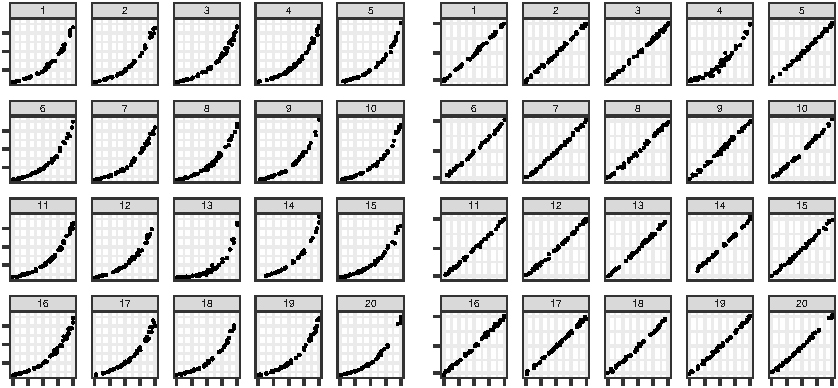
\includegraphics{jsm-2021-student-paper-submission_files/figure-latex/lineup-example-1} 

}

\caption{The plot on the left displays increasing exponential data on a linear scale with panel (2 x 5) + 3 as the target. The plot on the right displays increasing exponential data on the log scale with panel 2 x 2 as the target.}\label{fig:lineup-example}
\end{figure}

\hypertarget{data-generation}{%
\section{Data Generation}\label{data-generation}}

\textcolor{Plum}{
The most common type of lineup used in graphical experiments is a standard lineup containing one "target" dataset embeded within a set of null datasets. 
One way to generate the null datasets when working with real data is through the use of permutation. 
In this study, both the target and null datasets were generated by simulating data from an exponential model with differing parameters. 
This experiment was designed to test a participants ability to differentiate between different rates of exponential growth on both the log and linear scales. 
In order to gaurantee the simulated data spans the same range of values, we implemented a range constraint of $y\in [10,100]$ and a domain constraint of $x\in [0,20]$ with $N = 50$ points randomly assigned throughout the domain and mapped to the y-axis using the exponential model with the selected paramters. 
These constraints provide some assurance that participants who select the target plot are doing so because of their visual perception differentiating between curvature or slope rather than different starting or ending values. 
}

\hypertarget{exponential-model}{%
\subsection{Exponential Model}\label{exponential-model}}

\textcolor{Plum}{
We simulated data based on a 3-parameter exponential model with multiplicative errors. 
This model has a $\beta$ parameter to reflect the rate of growth and amount of curvature and $\sigma^2$ to reflect the amount of variability around the exponential growth curve. 
The parameters $\alpha$ and $\theta$ are adjusted based on $\beta$ and $\sigma^2$ to gauranee the range and domain constraints are met. 
The model generated $N = 50$ points $(x_i, y_i), i = 1,...,N$ where $x$ and $y$ have an increasing exponential relationship. 
The data was simulated heuristically by the following procedures:
}
\vspace{3 mm}

\textcolor{Plum}{\textit{Algorithm 2.1.1: Paremeter Estimation}}

\textcolor{Plum}{Input Parameters: domain $x\in[0,20]$, range $y\in[10,100]$, midpoint $x_{mid}$.}

\textcolor{Plum}{Output: estimated model parameters $\hat\alpha, \hat\beta, \hat\theta$}

\begin{enumerate}
\def\labelenumi{\arabic{enumi}.}
\item
  \textcolor{Plum}{Determine the $y=-x$ line scaled to fit the assigned domain and range.}
\item
  \textcolor{Plum}{Map the values $x_{mid} - 0.1$ and $x_{mid} + 0.1$ to the $y=-x$ line for two additional points.}
\item
  \textcolor{Plum}{From the set points $(x_k, y_k)$ for $k = 1,2,3,4$, obtain the coefficients from the linear model $\ln(y_k) = b_0 +b_1x_k$ to obtain starting values - $\alpha_0 = e^{b_0}, \beta_0 =  b_1, \theta_0 = 0.5\cdot \min(y)$}
\item
  \textcolor{Plum}{Using the `nls()` function from the `stats` package in Rstudio and the starting parameter values - $\alpha_0, \beta_0, \theta_0$ - fit the nonlinear model, $y_k = \alpha\cdot e^{\beta\cdot x_k}+\theta$ to obtain estimated parameter values - $\hat\alpha, \hat\beta, \hat\theta.$}
\end{enumerate}

\textcolor{Plum}{\textit{Alogrithm 2.1.2: Exponential Simulation}}

\textcolor{Plum}{Input Paremeters: sample size $N = 50$, estimated parameters $\hat\alpha$, $\hat\beta$, and $\hat\theta$, $\sigma$ standard deviation from the exponential curve.}

\textcolor{Plum}{Output Parameters: $N$ points, in the form of vectors $\mathbf{x}$ and $\mathbf{y}$.}

\begin{enumerate}
\def\labelenumi{\arabic{enumi}.}
\item
  \textcolor{Plum}{Generate $\tilde x_j, j = 1,..., N\cdot \frac{3}{4}$ as a sequence of evenly spaced points in $[0,20]$. This ensures the full domain of $x$ is used, fulfilling the constraints of spanning the same domain and range for each parameter combination.}
\item
  \textcolor{Plum}{Obtain $\tilde x_i, i = 1,...N$ by sampling $N = 50$ values from the set of $\tilde x_j$ values. This gaurantees some variability and potential clustring in the exponential growth curve disrupting the perception due to continuity of points.}
\item
  \textcolor{Plum}{Obtain the final $x_i$ values by jittering $\tilde x_i$.}
\item
  \textcolor{Plum}{Calculate $\tilde\alpha = \frac{\hat\alpha}{e^{\sigma^2/2}}.$ This ensures that the range of simulated values for different standard devaition parameters has an equal expected value for a given rate of change due to the non-constant variance across the domain.}
\item
  \textcolor{Plum}{Generate $y_i = \tilde\alpha\cdot e^{\hat\beta x_i + e_i}+\hat\theta$ where $e_i\sim N(0,\sigma^2).$}
\end{enumerate}

\hypertarget{parameter-selection}{%
\subsection{Parameter Selection}\label{parameter-selection}}

\textcolor{Plum}{
The exponential model provides the base for this graphical experiment. 
We manipulate the midpoint, $x_{mid}$, and in turn the estimated parameters to control the amount of curvature present in the data and the error standard deviation, $\sigma$, to control the amount of deviation from the exponential curve.
We selected three midpoints corresponding to difficulty levels easy (obvious curvature), medium (noticeable curvature), and hard (almost linear) along with a sensible choice of standard deviation, $\sigma$ (Table 1).
The midpoints and standard deviation combinations were chosen similar to in \cite{vanderplas_clusters_2017}. 
For each level of difficulty, we simulated 1000 datasets of $(x_{ij}, y_{ij})$ points for $i = 1,...,50$ and $j = 1...10$. 
Each generated $x_i$ point from \textit{Algorithm 2.1.2} was replicated 10 times.  
Then the lack of fit statistic (LOF) was computed for each simulated dataset by calculating the deviation of the data from a linear line. 
Plotting the density curves of the LOF statistics for each level of difficulty choice allows us to evalute the ability of differentiating between the difficulty levels and thus detecting the target plot.
In Figure \ref{fig:lof-density-curves}, we can see the densities of each of the three difficulty levels. 
While the LOF statistic provides us a numerical value for discriminating between the difficulty levels, we cannot directly realte this to the perceptual discriminability. 
}

\begin{table}

\caption{\label{tab:parameter-data}Exponential parameter selection}
\centering
\begin{tabular}[t]{ccccccc}
\toprule
 & $x_{Mid}$ & $\hat\sigma$ & $\hat\alpha$ & $\tilde\alpha$ & $\hat\beta$ & $\hat\theta$\\
\midrule
Obvious Curvature & 14.5 & 0.25 & 0.91 & 0.88 & 0.23 & 9.10\\
Noticable Curvature & 13.0 & 0.12 & 6.86 & 6.82 & 0.13 & 3.14\\
Almost Linear & 11.5 & 0.05 & 37.26 & 37.22 & 0.06 & -27.26\\
\bottomrule
\end{tabular}
\end{table}

\begin{figure}

{\centering 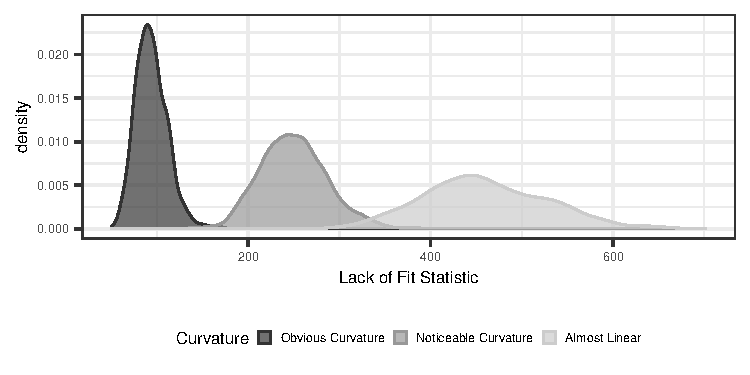
\includegraphics{jsm-2021-student-paper-submission_files/figure-latex/lof-density-curves-1} 

}

\caption{Density plot of the lack of fit statistic showing separation of difficulty levels: obvious curvature, noticable curvature, and almost linear.}\label{fig:lof-density-curves}
\end{figure}

\hypertarget{lineup-setup}{%
\subsection{Lineup Setup}\label{lineup-setup}}

\textcolor{Plum}{There were a total of three parameter combinations corresponding to the three difficulty levels - easy (obvious curvature), medium (noticeable curvature), and hard (almost linear). 
The lineup plots were generated by mapping simulating data corresponding to difficulty level A to a scatterplot while the null plots were generated by mapping simulated data corresponding to difficulty level B to a scatterplot. 
For exmaple, a target plot with simulated data following an increasing exponential curve with obvious curvature is embeded within null plots with simulated data following an increasing exponential that is almost linear (i.e. Easy-Hard). 
By our constraints, the target plot and null plots will span a similar domain and range. 
There are a total of 6 (i.e. 3 choose 2) lineup parameter combinations.
Two sets of each lineup parameter combination were simulated (total of 12 test datasets) and plotted on both the linear and the log scale (total of 24 test lineup plots). 
It is worth noting that there were also three rorschach lineup parameter combinations (e.g. Easy-Easy) and that each of these also had two sets of datasets simulated and plotted on both scales (12 rorscahch lineup plots). Evaluations of the rorscahch lineup plots were not included in the anaysis of this paper.
}

\hypertarget{study-design}{%
\subsection{Study Design}\label{study-design}}

\textcolor{Plum}{
Each participant was shown a total of thirteen lineup plots (twelve) test lineup plots and one rorschach lineup plot). Participants were randomly assigned one of the two replicate datasets for each of the six unique lineup parameter combinations. For each assigned test dataset, the participant was shown the lineup plot corresponding to both the linear scale and the log scale. For the additional rorschach lineup plot, participants were randomly assigned a rorschach dataset on either the linear or the log scale. The order of the thirteen lineup plots shown was randomized for each participant. 
}

\hypertarget{participant-recruitment}{%
\subsection{Participant Recruitment}\label{participant-recruitment}}

\textcolor{Plum}{Participants above age 19 were recruited from Reddit's R Visualization and R Sample Size communities.
Since participants recruitted on Reddit were not compensated for their time, most participants have an interest in data visualization research. 
Previous literature suggests that prior mathematical knowledge or experience with exponential data is not associated with the outcome of graphical experiments (CITE THIS!). 
Participants were then directed to complete the experimental task available at https://shiny.srvanderplas.com/log-study/.
}

\hypertarget{task-description}{%
\subsection{Task Description}\label{task-description}}

\textcolor{Plum}{Participants were shown a series of twelve test lineup plots and asked to identify the plot that was most different from the others. 
On each plot, participants were asked to justify their choice and provide their level of confidence in their choice.
The goal of this experimental task is to test an individuals ability to perceptually differentiate exponentially increasing data with differing rates of change on both the linear and log scale. 
In \cite{best_perception_2007}, the authors explored whether descrimination between curve types is possible. 
They found that accuracy higher when nonlinear trends presented (e.g. it’s hard to say something is linear, but easy to say that it isn’t) and that accuracy higher with low additive variability. We hypothesize log scales should make it much easier to estimate the growth rate since we estimate slopes relatively accurately, resolving much of the difficulty with exponential estimation \citep{mosteller_eye_1981}.
}

\hypertarget{results}{%
\section{Results}\label{results}}

\textcolor{Plum}{
Participant recruitment through Reddit occurred over the course of two weeks during which 58 individuals completed 518 unique test lineup evaluations. Participants who completed fewer than 6 lineup evaluations were removed from the study (17 participants, 41 evaluations). The final dataset included a total of 41 participants and 477 lineup evaluations. Each plot was evaluated between 18 and 28 individuals (Mean: 21.77, SD: 2.29). In 67% of the 477 lineup evaluations, participants correctly identified the target panel.
}
\textcolor{Plum}{
Target plot identification was anlalyzed using the Glimmix Procedure in SAS 9.4. Each lineup plot evaluated was assigned a value based on the participant response (correct = 1, not correct = 0). Define $Y_{ijkl}$ to be the event that participant $l$ correctly identifies the target plot for dataset $k$ with curvature $j$ plotted on scale $i$. The binary response was analyzed using generalized linear mixed model following a binomial distribution with a logit link function following a row-column blocking design accounting for the variation due to participant and dataset respectively with a split plot design accounting for the same participant evaluating the same dataset on both the linear scale and log scale as shown in the Equation (1).
\begin{equation}
\text{logit }P(Y_{ijk}) = \eta + \delta_i + \gamma_j + \delta \gamma_{ij} + s_l + d_k + wp_{jkl}
\end{equation}
where
\begin{align*}
&\eta               \text{ is the beaseline average probability of selecting the target plot.} \\
&\delta_i           \text{ is the effect of the log/linear scale.} \\
&\gamma_j           \text{ is the effect of the curvature combination.} \\
&\delta\gamma_{ij}  \text{ is the two-way interaction effect of the scale and curvature.} \\
&s_l \sim N(0,\sigma^2_\text{{participant}}), \text{ random effect for participant characteristics} \\
&d_k \sim N(0,\sigma^2_{\text{dataset}}), \text{ random effect for data specific characteristics.} \\
&wp_{jkl} \sim N(0,\sigma^2_\text{{whole-plot}}), \text{ random effect for the particular participant by dataset charactersitics.}
\end{align*}
We assume that random effects for dataset, participant, and whole plot effects are independent. ADD MODEL DETAILS TO APPENDIX?
}

\begin{figure}
\centering
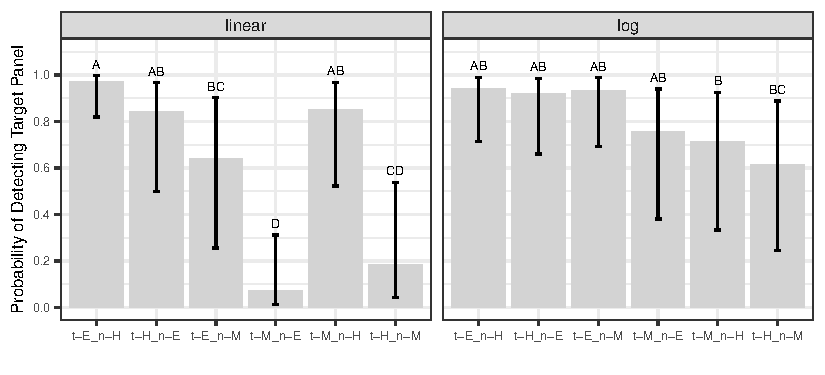
\includegraphics{jsm-2021-student-paper-submission_files/figure-latex/lsmeans-plot-1.pdf}
\caption{Least Squares Means}
\end{figure}

\begin{figure}
\centering
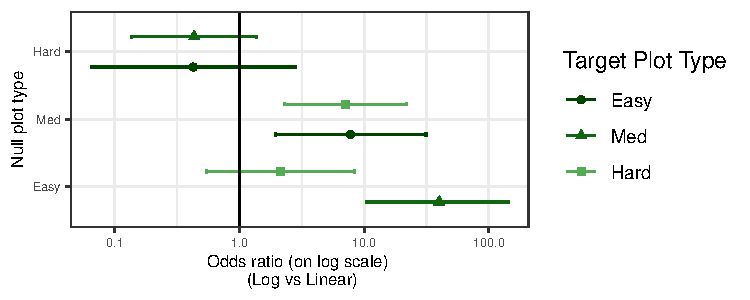
\includegraphics{jsm-2021-student-paper-submission_files/figure-latex/odds-ratio-plot-1.pdf}
\caption{Odds Ratio's}
\end{figure}

\hypertarget{discussion-and-conclusion}{%
\section{Discussion and Conclusion}\label{discussion-and-conclusion}}

\textcolor{Plum}{
In this study, we discovered that differentiation between data following exponentially increasing trends with differing growth rates is FINISH THIS.
}

\textcolor{Plum}{
Further experimentation is necessary to test an individual's ability to make predictions for exponentially increasing data. 
Previous literature suggests that we tend to underestimate predictions of exponentially increasing data.\citep{jones_generalized_1979, jones_polynomial_1977, wagenaar_extrapolation_1978}.
\citep{mosteller_eye_1981} designed and carried out an empirical investigation to explore properties of lines fitted by eye.
The researchers found that students tended to fit the slope of the first principal component or major axis (the line that minimizes the sum of squares of perpendicular rather than vertical distances) and that students who gave steep slopes for one data set also tended to give steep slopes on the others. 
Interestingly, the individual-to-individual variability in slope and in intercept was near the standard error provided by least squares.
A similar graphical taxk is used in the New York Times "You Draw It" page asking readers to test their knowledge by using their curser to estimate values of a certain topic under different political administrations or over different years (CITE THIS).
In addition to differentiation and prediction of exponentially increasing data, it is of interest to test an individuals ability to translate a graph of exponentially increasing data into real value quantities and extend their estimations by making comparisons. 
\citep{friel_making_2001} emphasize the importance of graph comprehension proposing that the graph construction plays a role in the ability to read and interpret graphs.
}

\hypertarget{supplementary-materials}{%
\section*{Supplementary Materials}\label{supplementary-materials}}
\addcontentsline{toc}{section}{Supplementary Materials}

\begin{itemize}
\item
  \textcolor{Plum}{\textbf{Code:} R code to reproduce figures of the article as well as SAS code to fit models used in the article. (\href{https://github.com/srvanderplas/Perception-of-Log-Scales/blob/master/manuscripts/jsm-2021-student-paper-submission/code/image-generator.R}{image-generator.R}, R file; \href{https://github.com/srvanderplas/Perception-of-Log-Scales/blob/master/lineups-pilot-analysis/sasCode/glmm-analysis-jsm-student-paper.sas}{glmm-analysis-jsm-student-paper.sas}, SAS file)}
\item
  \textcolor{Plum}{\textbf{Data:} Anonymized responses from the Reddit study to investigate the use of logarithmic scales. Each line corresponds to one lineup evaluation by a participant. (\href{https://github.com/srvanderplas/Perception-of-Log-Scales/blob/master/lineups-pilot-analysis/data/jsm-student-paper-11302020.csv}{jsm-student-paper.csv}, csv file)}
\end{itemize}

\hypertarget{acknowledgements}{%
\section*{Acknowledgement(s)}\label{acknowledgements}}
\addcontentsline{toc}{section}{Acknowledgement(s)}

\textcolor{Plum}{I gratefully acknowledge Dr. Susan VanderPlas and Dr. Reka Howard for their compuatational and statistical guidance. All data collection has been conducted with approval from the University of Nebraska - Lincoln Institutional Review Board (UNL IRB).}

\bibliographystyle{tfcad}
\bibliography{references.bib}




\end{document}
